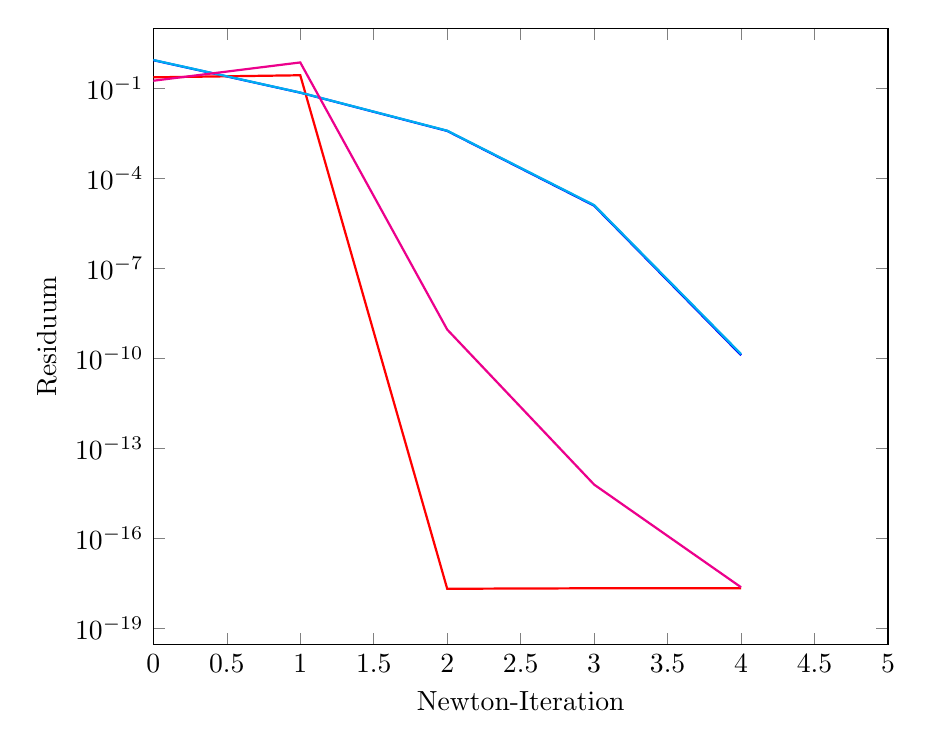
\begin{tikzpicture}[every plot/.append style={thick}] 
\begin{axis}[ 
label style={font=\normalsize}, 
xlabel={Newton-Iteration}, 
ylabel={Residuum}, 
xmin=0, xmax=5, 
ymode=log, 
ymin=0, ymax=10, 
width=0.9\textwidth, 
grid style=dashed, 
] 
\addplot[ 
color=blue, 
] 
coordinates { 
(0, 8.62e-01)(1, 7.12e-02)(2, 3.78e-03)(3, 1.22e-05)(4, 1.27e-10)}; 
\addplot[ 
color=red, 
] 
coordinates { 
(0, 2.31e-01)(1, 2.71e-01)(2, 2.10e-18)(3, 2.18e-18)(4, 2.17e-18)}; 
\addplot[ 
color=cyan, 
] 
coordinates { 
(0, 8.76e-01)(1, 7.19e-02)(2, 3.86e-03)(3, 1.28e-05)(4, 1.39e-10)}; 
\addplot[ 
color=magenta, 
] 
coordinates { 
(0, 1.78e-01)(1, 7.25e-01)(2, 9.11e-10)(3, 6.21e-15)(4, 2.35e-18)}; 
\end{axis} 
\end{tikzpicture} 
